\section{Aproximace hodnoty obrazové funkce při geometrických transformacích diskrétních obrazů}
Při geometrických transformacích diskrétních obrazů je nutné aproximovat hodnotu obrazové funkce $f(x,y)$. Proč? Uveďte 
alespoň dvě metody pro takovou aproximaci (nejlépe obrázkem, vzorcem, \dots).

Uvažujme příklad, kdy máme diskrétní obraz. Ten má ale hodnoty definované jen pro celá čísla, jako (15, 32) nebo 
(16, 33). Hodnotu pro bod (15.7, 32.2) neznáme. Proto musíme jeho barvu či jas odhadnout z okolních bodů, jejichž 
hodnoty známe. Tento proces odhadu se nazývá interpolace.

\begin{multicols}{2}
    \begin{figure}[H]
        \begin{tikzpicture}[scale=2.5]
            % grid & axis
            \draw[step=1, gray, very thin] (-0.5,-0.5) grid (1.5,1.5);
            \node at (-0.5, 1) [left] {};
            \node at (1, -0.5) [below] {};

            % pixels
            \fill[black] (0,0) circle (2pt) node[below left] {$P(15,32)$};
            \fill[black] (1,0) circle (2pt) node[below right] {$P(16,32)$};
            \fill[black] (0,1) circle (2pt) node[above left] {$P(15,33)$};
            
            % picked nearest neighbour
            \fill[red] (1,1) circle (2pt) node[above right, red] {$P(16,33)$};
            
            % point to interpolate
            \fill[blue] (0.7, 0.8) circle (2pt) node[below=0.5em] {$P(15.7,32.8)$};
            
            \draw[-Stealth, thick, blue] (0.7, 0.8) -- (0.95, 0.95);
        \end{tikzpicture}
        \caption{Interpolace nejbližšího souseda}
    \end{figure}

    \begin{figure}[H]
        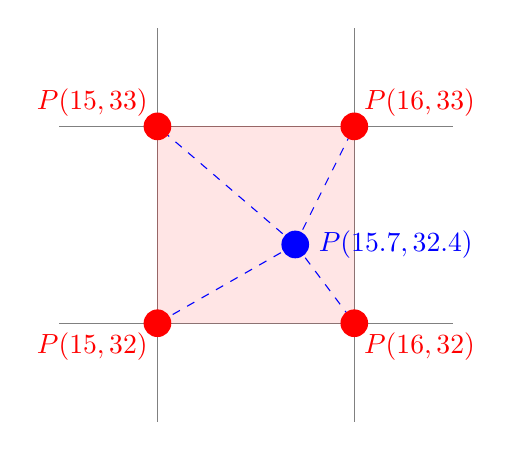
\begin{tikzpicture}[scale=2.5]
            % grid & axis
            \draw[step=1, gray, very thin] (-0.5,-0.5) grid (1.5,1.5);
            \node at (-0.5, 1) [left] {};
            \node at (1, -0.5) [below] {};
            
            % 2x2 area
            \draw[red, fill=red, opacity=0.1] (0,0) rectangle (1,1);
            
            % point to interpolate
            \fill[blue] (0.7, 0.4) circle (2pt) node[right=0.5em] {$P(15.7,32.4)$};
            
            % dependency on 4 neighbours
            \draw[dashed, blue] (0.7, 0.4) -- (0,0);
            \draw[dashed, blue] (0.7, 0.4) -- (1,0);
            \draw[dashed, blue] (0.7, 0.4) -- (0,1);
            \draw[dashed, blue] (0.7, 0.4) -- (1,1);

            % pixels
            \fill[red] (0,0) circle (2pt) node[below left, red] {$P(15,32)$};
            \fill[red] (1,0) circle (2pt) node[below right, red] {$P(16,32)$};
            \fill[red] (0,1) circle (2pt) node[above left, red] {$P(15,33)$};
            \fill[red] (1,1) circle (2pt) node[above right, red] {$P(16,33)$};
        \end{tikzpicture}
        \caption{Bilineární interpolace}
    \end{figure}

\end{multicols}
